\section{Verwendung und Umfeld des JHelioviewers}
Wie der Name bereits verrät ist JHelioviewer eine Applikation,  die zur Analyse von Sonnendaten verwendet wird. Es wird international zur Sonnenforschung eingesetzt und wird von der FHNW zusammen mit der ESA entwickelt. Momentan ist eine neue Version des JHelioviewer in Entwicklung, welche die Sonne im dreidimensionalen Raum darstellt. Ein Feature von JHelioviewer ist die Magnetfeldlinien darzustellen und zu animieren, die Abbildung \ref{einleitung::feldlinien} zeigt die Visualisierung.
\begin{figure}[!htbp]
\center
	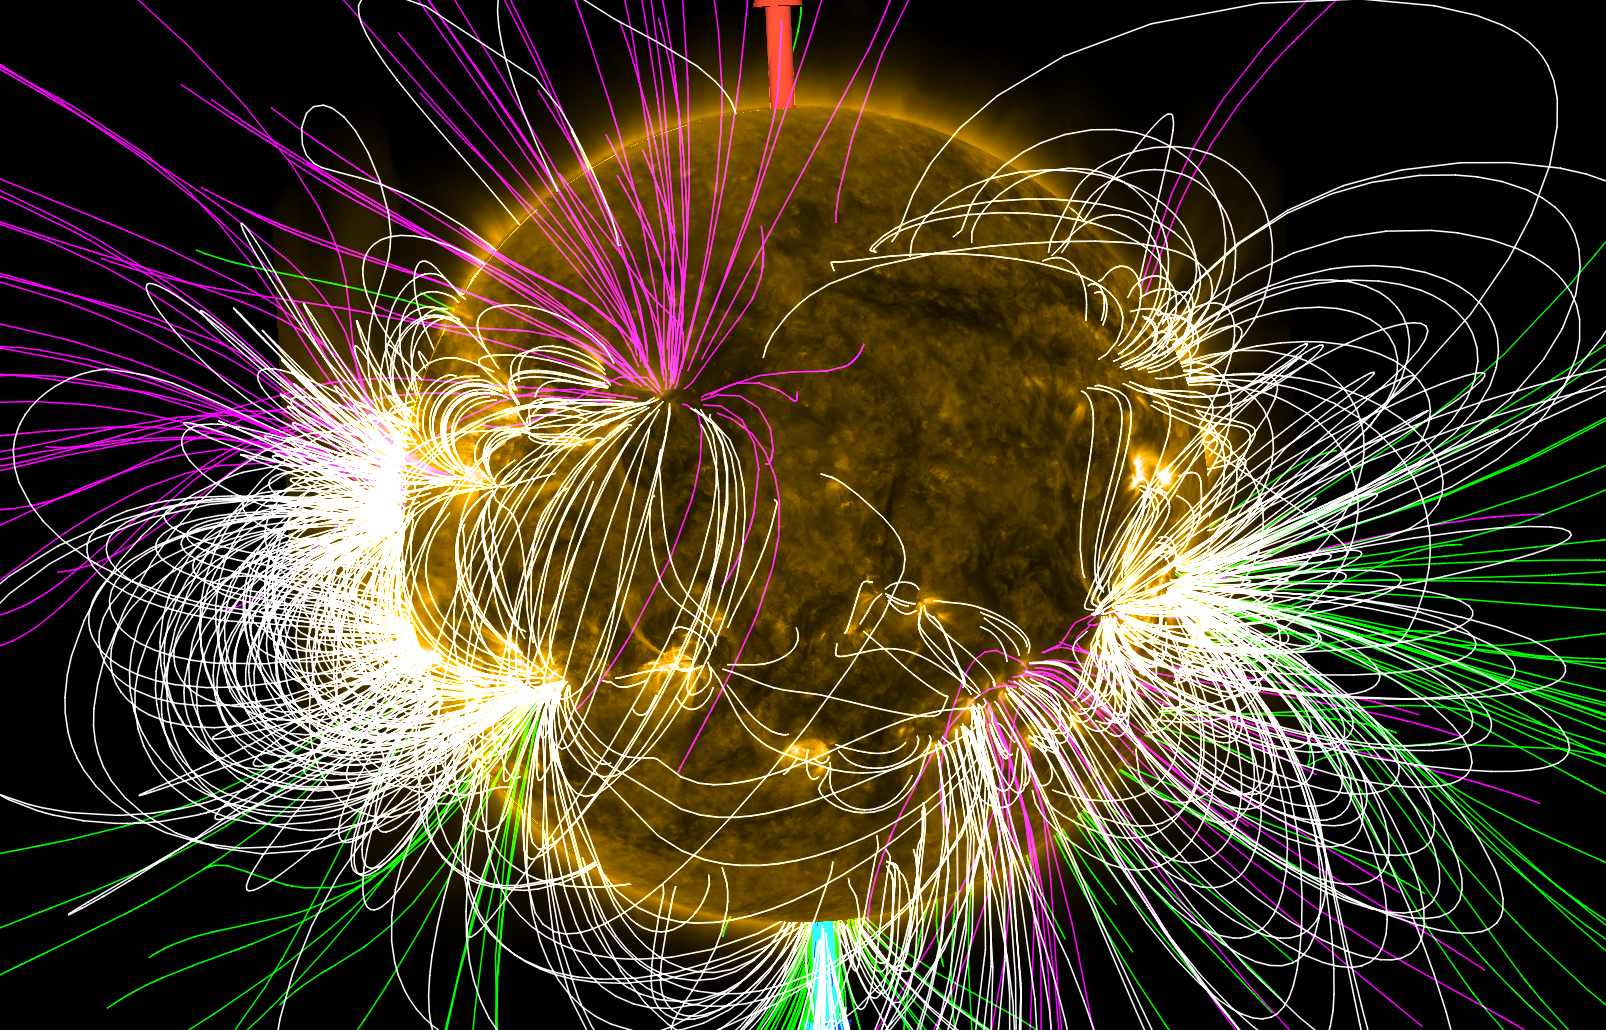
\includegraphics[width=0.8\textwidth,height=8cm,keepaspectratio]{./pictures/einleitung/fieldLines.png}
	\caption{Visualisierung der Feldlinien im JHelioviewer}
	\label{einleitung::feldlinien}
\end{figure}
Es wird zwischen drei Feldlinien Unterschieden: Linien, die auf der Sonne starten und wieder auf der Sonne landen, auf der Sonne starten und ins Weltall führen oder vom Weltall auf der Sonne landen. Die weissen Feldlinien repräsentieren ''Sonne zu Sonne´´, die Grünen ''Sonne zu Weltall´´ und die Violetten ''Weltall zu Sonne´´. Die Feldlinien sind, allgemein Betrachtet, eine grosse Menge an Punkten, welche ein Server bereitstellt. Die Abbildung \ref{einleitung::aufbau} visualisiert den Datenfluss.
\begin{figure}[!htbp]
\center
	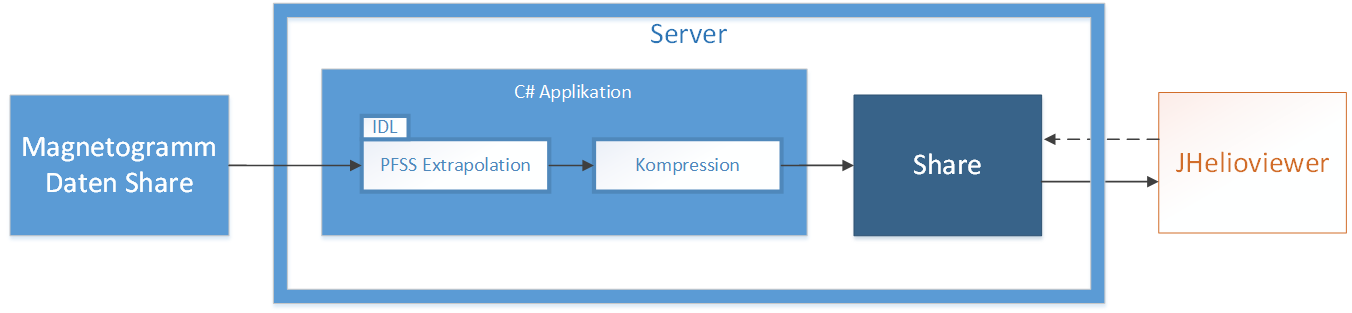
\includegraphics[width=0.8\textwidth,height=6cm,keepaspectratio]{./pictures/einleitung/server.png}
	\caption{Aufbau und Datenfluss des Servers}
	\label{einleitung::aufbau}
\end{figure}
In regelmässigen Abständen sucht der Server nach neuen Oberflächen-Magnetogramm-Daten der Satelliten. Alle sechs Stunden wird die Oberfläche der Sonne neu gemessen.Daraus werden mittels Potential Field Source Surface (PFSS) Extrapolation die Feldlinien zu diesem Zeitpunkt errechnet. Danach führt der Server eine verlustlose Kompression durch und stellt die Daten auf einem öffentlichen Share dem JHelioviewer zur Verfügung. Der JHelioviewer lädt dann zur Laufzeit die Feldlinien, die er benötigt.\\[\baselineskip]
Jede halbe Stunde schiesst ein Satellit ein Bild der Sonne. Wenn der JHelioviewer also einen Zeitraum animieren soll, existiert für jede halbe Stunde ein Bild der Sonne, eine Aufnahme des Magnetfelds existiert aber nur alle sechs Stunden eine Simulation. Bei einer Animation gibt es also nur für jedes zwölfte Bild neue Feldlinien. Durch den grossen Zeitabstand und durch die Eigenschaften der PFSS Extrapolation unterscheiden sich die Feldlinien stark von Simulation zu Simulation. Das führt zu einem schlagartigen Wechsel in der Animation. In der Zukunft soll dieser schlagartige Wechsel behoben werden, indem beispielsweise die PFSS Extrapolation in kürzeren Intervallen berechnet wird, oder durch Interpolation von einer Feldlinien-Simulation zur Anderen.

\subsection{Rohdatenmenge der Feldlinien}
Die PFSS Extrapolation produziert für eine Aufnahme etwa 15 MiBytes an Daten. Wenn man annimmt, dass für jedes zwölfte Bild eine Aufnahme existiert und der JHelioviewer bei 60 Bilder in der Sekunde animiert, muss eine Aufnahme in etwa 0.2 Sekunden heruntergeladen und angezeigt werden. Wenn man noch beachtet, dass der Server vermutlich nicht lokal, sodern nur über eine Internetverbindung erreichbar ist, ist eine Animation mit dieser Datenmenge nicht möglich. Deshalb wurde bereits die Datenmenge verkleinert auf etwa 1.5 MiBytes pro Aufnahme. Aber auch das ist noch zu gross. Der JHelioviewer müsste eine konstante Geschwindigkeit um die 60 MiBit haben. Ziel dieser Arbeit ist deshalb eine Kompression zu entwickeln, welche eine flüssige Animation erlaubt.

\subsection{Komprimierung mittels verlustloser und verlustbehafteten Ansätzen}
Verlustlos:Kein Datenverlust, aber nur begrenzte komprimierung (shannons source code theorem?)
Datenmenge bereits im Vorfeld  mit verlustbehafteten und verlustlosen Ansätzen verringert.
mehr verlustbehaftet aber in guter Qualität


 